%!TEX root=masterproef.tex

\subsection{Attesteren van software}
\label{subsection:attestation}

Het voorbeeld uit sectie \ref{section:node-capture} toonde al aan dat zelfs het
vluchtige geheugen van een knoop niet veilig is. Als een aanvaller in staat is
om ongemerkt de programma-code van een knoop te bekomen, alsook alle gegevens
die alleen tijdens uitvoering in het geheugen, dan kan deze aanvaller deze code
aanpassen zodat de werking ogenschijnlijk ongewijzigd is, maar dat hij toch
controle heeft over de werking en zo het hele netwerk kan be\"invloeden.

Een zeer logische onderzoeksvraag dient zich al snel aan: ``\emph{Is het
mogelijk om wijzigingen aan het programma van een knoop in het netwerk vast te
stellen?}''. Deze vraag wordt onderzocht binnen het domein van software
attestatie.

\subsubsection*{Werking}

Alle bestaande vormen van software attestatie maken gebruik van een protocol
gebaseerd op het challenge response principe. Als men de integriteit van een
knoop wil vast stellen, zal men aan deze knoop een verzoek sturen om een unieke
samenvatting te maken van zijn inhoud door middel van een cryptografische
hashfunctie, een \emph{checksum}.

De vaststeller beschikt zelf over een versie van de inhoud van de knoop en kan
dezelfde unieke samenvatting berekenen. Door in het initi\"ele verzoek een
\'e\'enmalig te gebruiken code mee te geven, een zgn. \emph{nonce}, en deze
deel te laten uitmaken van de inhoud, kunnen verschillende verzoeken telkens
met een ander, unieke samenvatting beantwoord worden en wordt kan deze
samenvatting niet op voorhand gekend en berekend worden. Figuur
\ref{fig:attestation-process} geeft een overzicht van de werking van software
attestatie en illustreert hoe een wijziging door een aanvaller zich propageert.

\begin{figure}[ht]
  \centering
  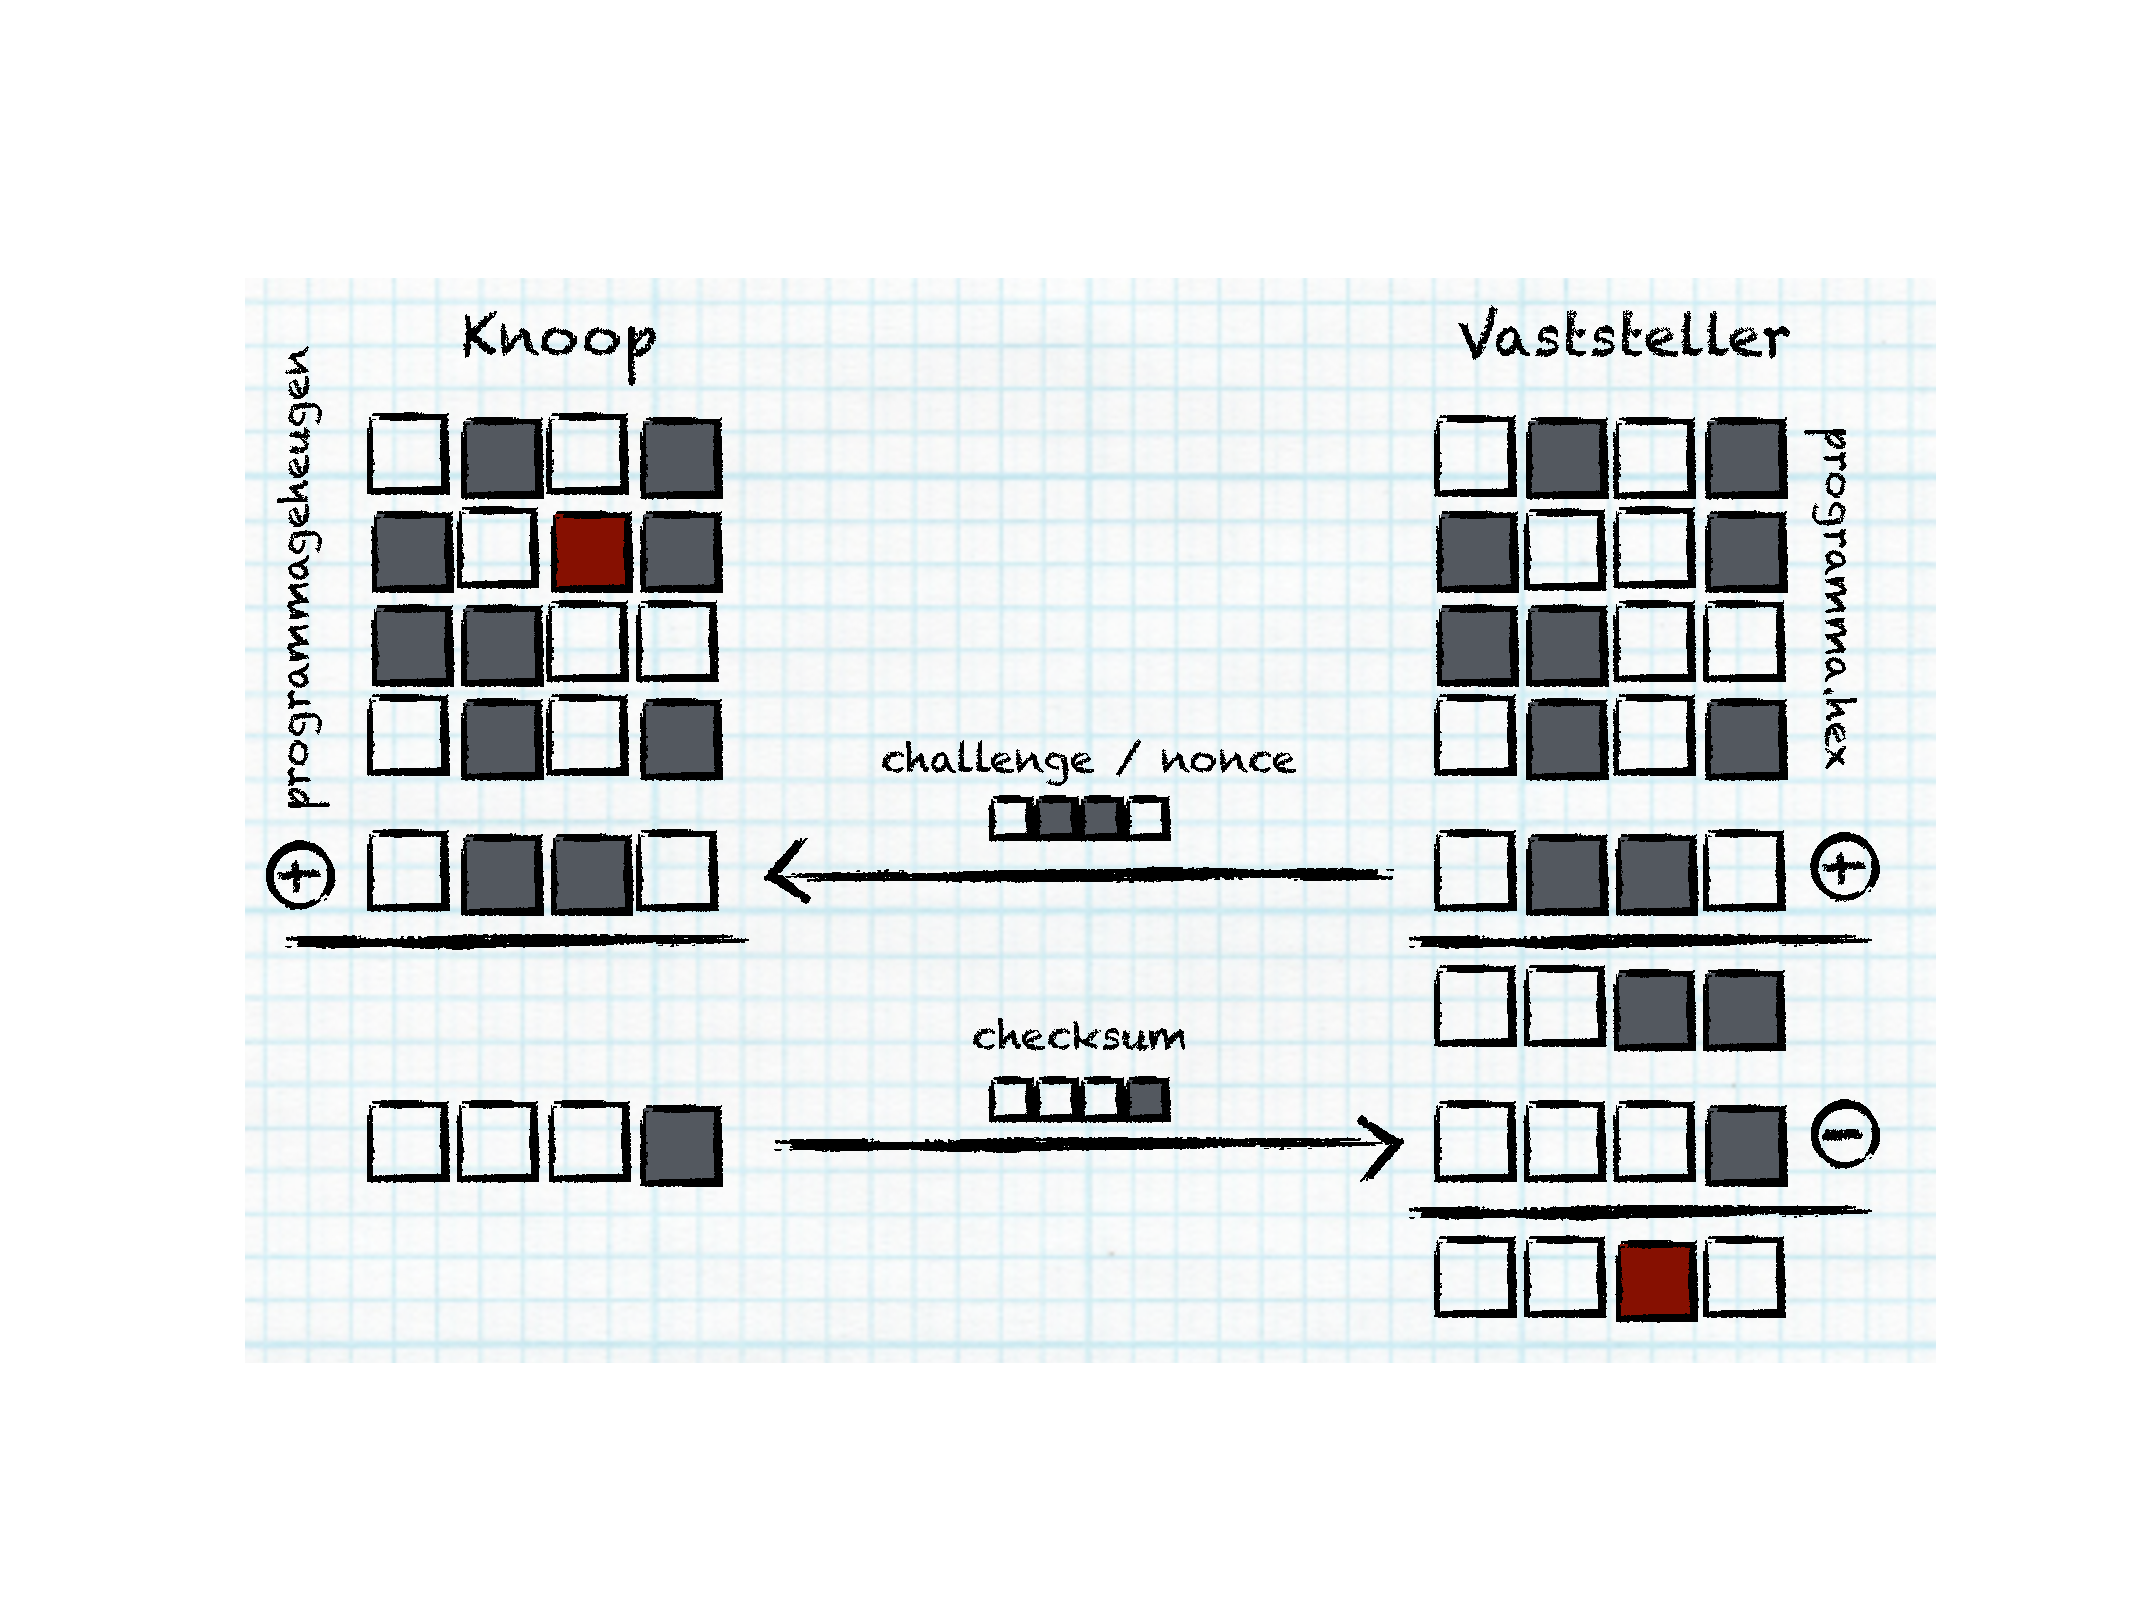
\includegraphics[width=0.9\linewidth]{resources/attestation-process.pdf}
  \caption{De werking van software attestatie: een aanvaller heeft een
  wijziging kunnen aanbrengen in de programma code op een knoop. Deze wijziging
  propageert zich in de \emph{checksum} en wordt door de vaststeller opgemerkt.}
  \label{fig:attestation-process}
\end{figure}

De inhoud waarvan een samenvatting gemaakt wordt is typisch de programma code
die op de knoop ge\"installeerd werd. Indien een aanvaller deze code kon
wijzigen, zou de samenvatting niet langer overeenkomen met die opgesteld door
de vaststeller en kan deze laatste besluiten om deze gewijzigde code niet te
vertrouwen en de knoop uit te sluiten.

\subsubsection*{Implementaties}

SWATT werd voorgesteld in \citep{seshadri2004swatt}. Het is een attestatie
procedure die een \emph{checksum} berekent over nagenoeg alle geheugenlocaties,
echter wel in willekeurige volgorde. Anderzijds houdt SWATT ook rekening houdt
met de tijd die de attestatie routine op de knoop nodig heeft om de
\emph{checksum} te berekenen. Indien een aanvaller code zou toevoegen om de
werking van de attestatie routine te verstoren, zou op te merken zijn in een
vertraging.

Met SCUBA in \citep{seshadri2006scuba} en SAKE in \citep{seshadri2008sake} werd
verder gebouwd op de SWATT techniek met het oog op een beveiligde distributie
van programma code en het veilig uitwisselen van sleutels. Samen met SCUBA en
SAKE werd ook \emph{Indisputable Code Execution} of ICE ge\"introduceerd. Daar
waar SWATT gericht is op inhoudelijke integriteit, voegt ICE hieraan ook de
garantie van een niet aangetaste uitvoering van programma's aan toe en laat het
toe om beperkte regio's van het geheugen te benaderen.

Op deze manier kan nu bovenop de attestatie van het geheugen van een knoop, nu
ook functionaliteit aangeroepen worden, waarvan de werking ook gegarandeerd
veilig is. Het installeren van nieuwe code en het uitwisselen van gedeelde
geheimen wordt op die manier mogelijk.

ICE realiseert dit door een \emph{checksum} te berekenen over de geheugenregio
waar de attestatie routine zich bevindt, alsook over de regio waar het uit te
voeren programma staat en van de staat van de processor. Hierdoor ontstaat er
een garantie dat de attestatie correct verloopt, dat het uit te voeren
programma geen onbekende code bevat en dat de omgeving waarin de attestatie en
het programma uitgevoerd worden gegarandeerd niet aangetast kan worden.

Een belangrijke eigenschap van de ICE techniek is dat de attestatie routine de
processor in een emph{veilige} staat brengt door geen interrupts toe te laten.
Hierdoor kan de werking van de attestatie routine niet onderbroken en gewijzigd
worden. Na correcte attestatie zal het geattesteerde programma in dezelfde
veilige omstandigheden als de ICE routine uitgevoerd worden.

\subsubsection*{Evaluatie}

De beweringen rond SWATT en ICE werden in \citep{castelluccia2009difficulty}
onder de loep genomen en verschillende manieren om deze vormen van
integriteits-controle te omzeilen werden voorgesteld. Ondanks het feit dat
verschillende interessante aspecten van de attestatie technieken werden
belicht, werden te snel veronderstellingen rond beide implementaties gemaakt en
werd in \citep{perrig2010refutation} een weerwoord gegeven.

Desalniettemin zijn de ontwijkingstechnieken die voorgesteld werden zeer
interessante voorbeelden van de mogelijkheden die een aanvaller heeft tegen
software attestatie. Het feit dat de op het eerste zicht inderdaad valabele
aanvallen toch nog fouten bevatten, biedt dan weer een ander interessant beeld
op de kwaliteiten van de voorgestelde technieken. We belichten ze in de
volgende paragrafen als inspiratiebron.

De fundamentele manier om de attestatie code te omzeilen bestaat er in om de
opgevraagde geheugenadressen te controleren en indien ze verwijzen naar
plaatsen waar zich niet-originele code bevindt, deze te herschrijven naar
adressen waar de originele code zich bevindt.

Aangezien het merendeel van het programma geheugen op een knoop typisch leeg
is, kan de aanvaller zijn benodigde code verbergen in zo'n stuk leeg geheugen.
Mits zorgvuldige keuze van deze locatie, kan het controleren van en verwijzen
naar een andere locatie zich beperken tot de manipulatie van \'e\'en enkele bit
in het adres. Deze techniek wordt ook wel een geheugen schaduwende aanval
genoemd.

Om het probleem van leeg programma geheugen en de bijhorende uitnodiging aan
het adres van de aanvaller om zich eenvoudig te kunnen verschuilen, aan te
pakken, stelelen o.a. \citep{yang2007distributed,seshadri2008sake} voor om dit
geheugen voor dat het op een knoop wordt geplaatst, op te vullen met
willekeurige waarden. Op deze manier heeft de aanvaller geen vrije ruimte om
zijn code in te plaatsen.

Ofschoon deze willekeurige data inderdaad zo kan opgesteld worden dat ze niet
kan verkleind worden, kan dit niet gegarandeerd worden van de eigenlijke
programma code. Deze kan typisch wel nog verkleind worden en in die vorm
opgeslagen worden, waardoor er mogelijk voldoende ruimte vrijkomt voor de code
van de aanvaller. Op het ogenblik van attestatie kan deze oorspronkelijke code
dan, indien nodig terug hersteld worden.

Indien deze eenvoudige technieken toch niet voldoende ruimte zouden bieden, kan
er nog altijd gekeken worden naar het data geheugen. We merken immers op dat
nagenoeg alle vormen van attestatie alleen toegepast worden op het programma
geheugen. Het data geheugen is immers te veranderlijk en kan niet volledig
gekend zijn door de vaststeller.

Hierdoor wordt dit data geheugen natuurlijk het volgende mogelijke
aandachtspunt voor de aanvaller. Ondanks het feit dat ook op een \mcu het data
geheugen veelal niet kan uitgevoerd worden, blijft het mogelijk om programma
code in het data geheugen op te slagen en te kopi\"eren naar het programma
geheugen.

De \emph{rootkit} voorgesteld in \citep{castelluccia2009difficulty} hanteert dit
principe. Door middel van de \emph{Return Operation Programming} (ROP)
techniek, o.a. beschreven in \citep{prandini2012return}, kan een aanvaller met
eerste haak bij aanvang van de attestatie code in het programma geheugen, zijn
eigen rootkit uit het programma geheugen laten verwijderen. Na deze operatie is
het programma geheugen opnieuw intact en zal de originele attestatie routine
een positief resultaat opleveren. Maar de eerste haak heeft er ook voor gezorgd
dat de bij terugkeer uit de attestatie routine een tweede haak geplaatst is die
op zijn beurt de rootkit en de initi\"ele haak opnieuw door middel van ROP
instructies installeert. Figuur \ref{fig:attestation-rootkit} toont deze
werking.

\begin{figure}[ht]
  \centering
  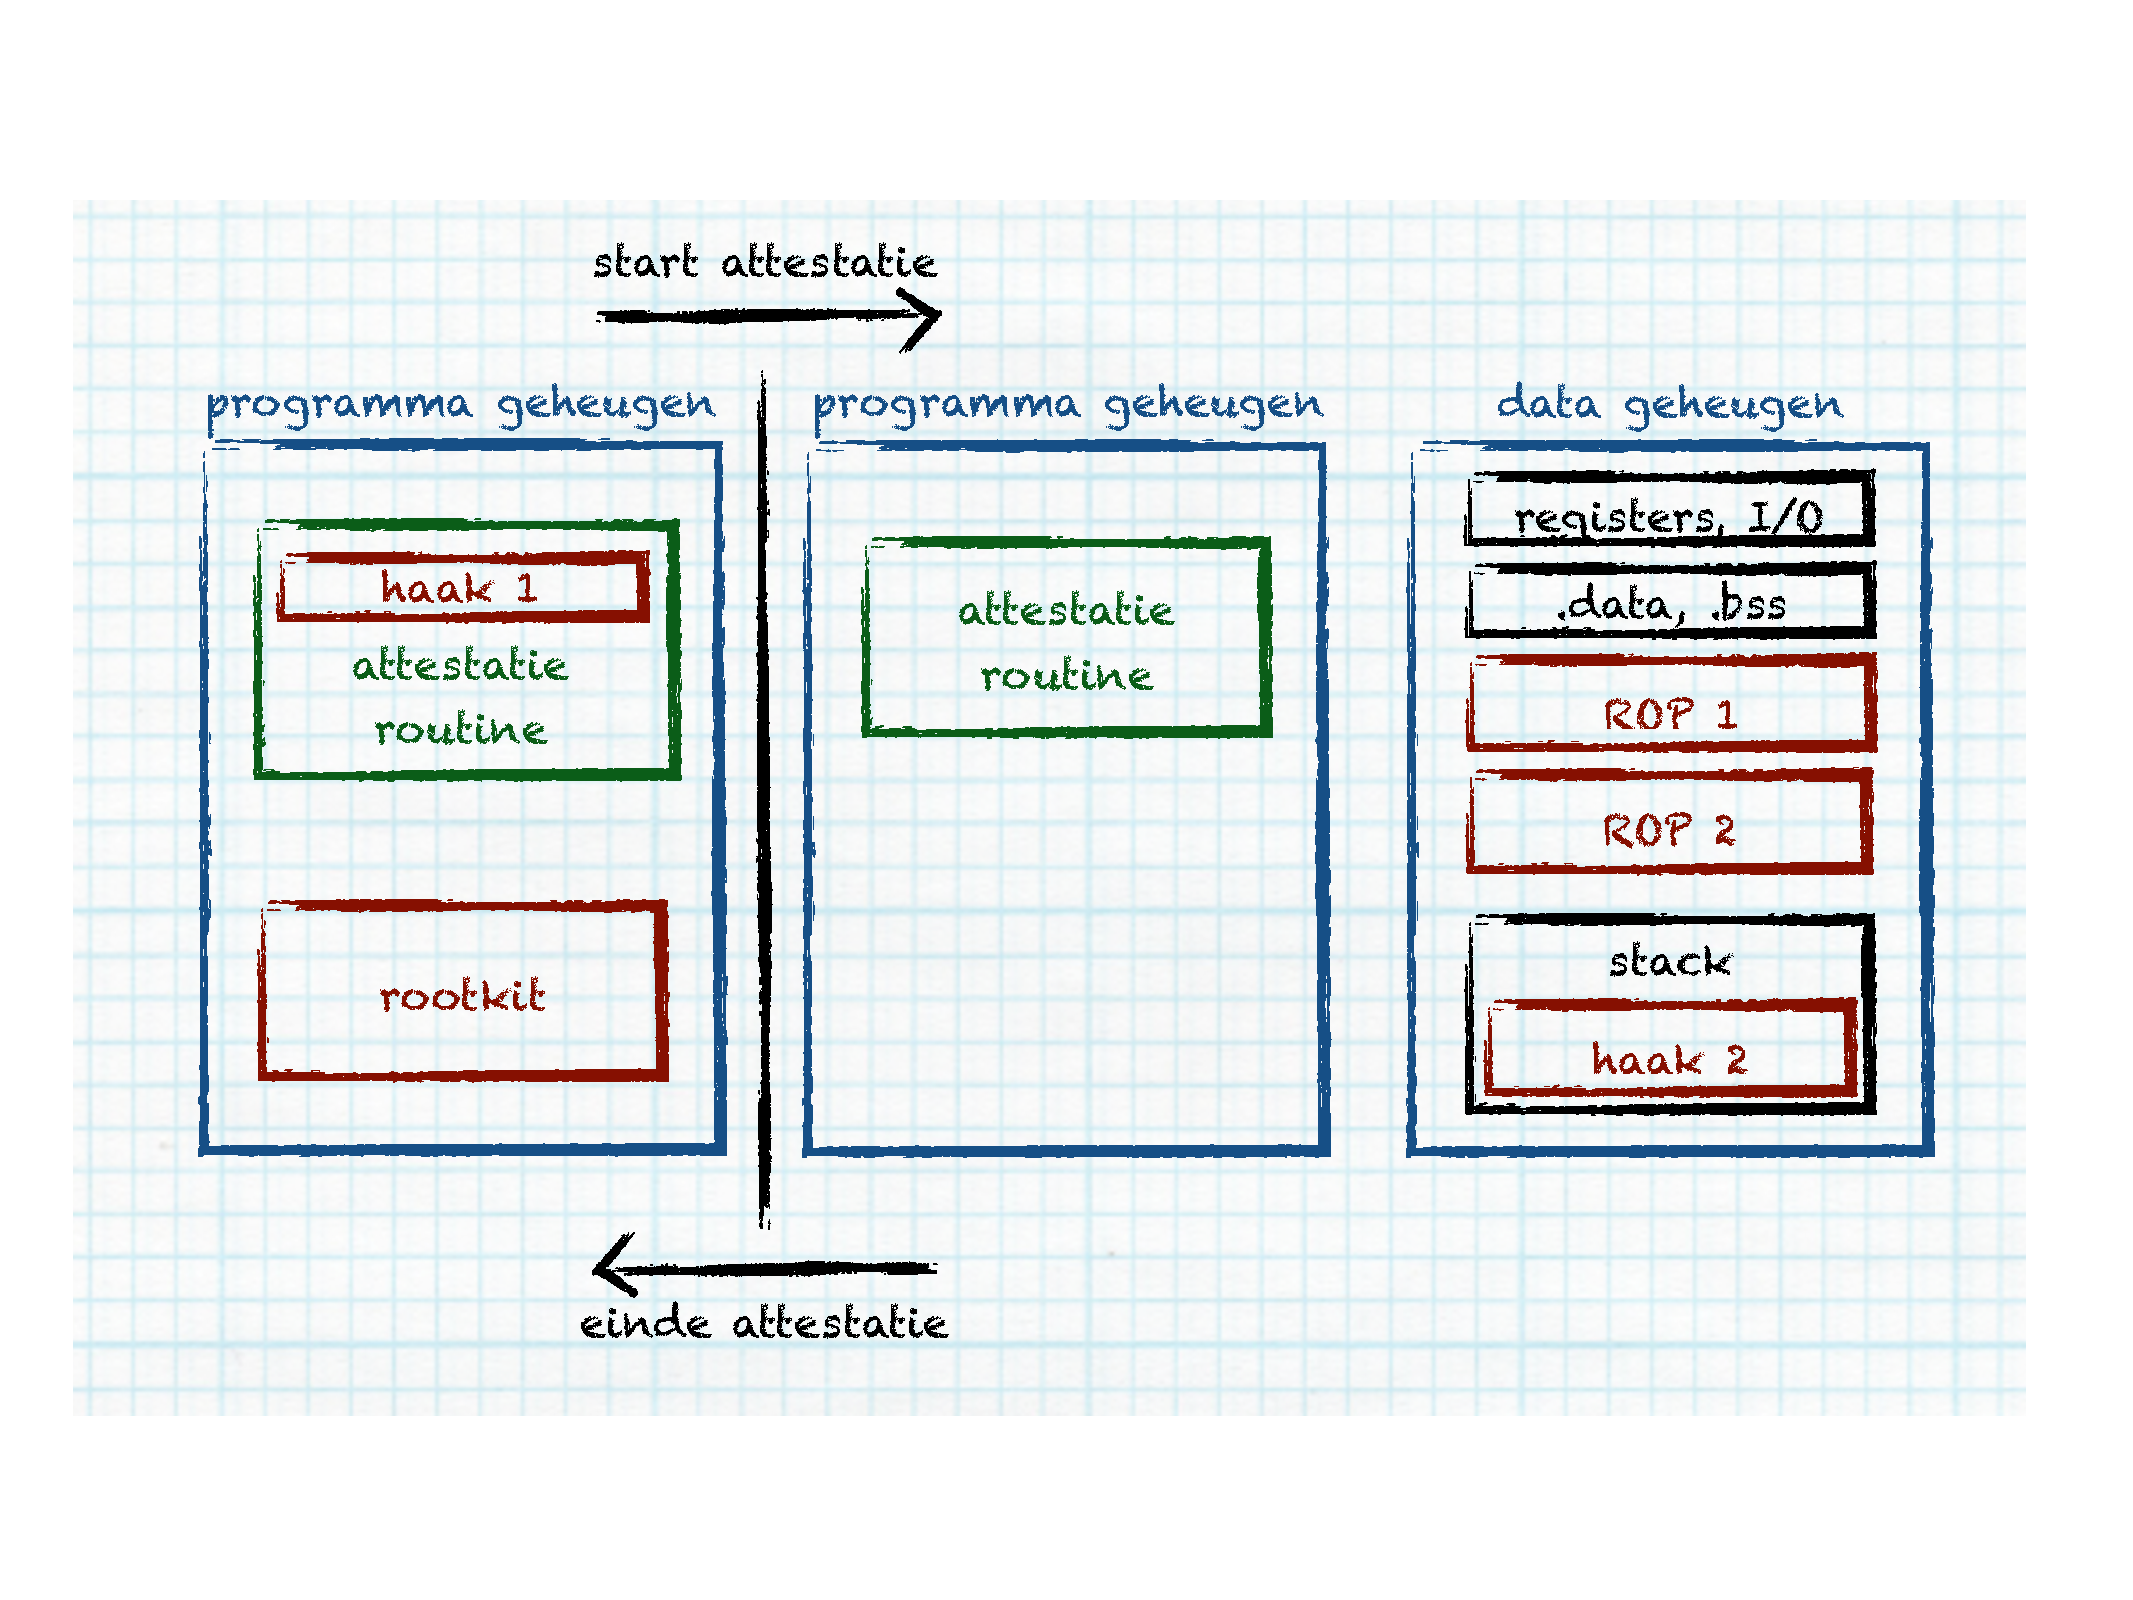
\includegraphics[width=0.9\linewidth]{resources/attestation-rootkit.pdf}
  \caption{De werking van een attestatie ontwijkende rootkit.}
  \label{fig:attestation-rootkit}
\end{figure}

Het verbergen van de rootkit en het herstellen van het programma geheugen in
zijn oorspronkelijke staat blijkt slechts een overhead van ongeveer 0.3\% op te
leveren t.o.v. bv. de SWATT attestatie techniek voorgesteld in
\citep{seshadri2004swatt}. Deze techniek controleert tevens de tijd dat de
attestatie routine nodig had om de checksum te berekenen. Indien deze te lang
duurt dan schrijft SWATT dit toe aan de overhead ge\"introduceerd door
mogelijke kwaadaardige code. Een verhoging met 0.3\% is mogelijk te weinig om
tot deze conclusie te komen.

Deze aanval richt zich nu louter op de attestatie routine, maar zoals in
\citep{perrig2010refutation} aangegeven wordt, it SWATT slechts een deel van een
volledige software attestatie en focust zich op het effectief attesteren van
code in het geheugen, niet op de omringende context. In een volledige
opstelling zou een attestatie procedure de het terugkeer adres op de stack mee
kunnen nemen in de attestatie.

\citep{castelluccia2009difficulty} beschrijven zelf enkele mogelijke pistes
waarmee een attestatie routine zichzelf zou kunnen beschermen tegen een
dergelijke rootkit. Een eerste zou op het einde van zijn implementatie het data
geheugen volledig leeg kunnen maken en vervolgens, zonder een terugkeer
operatie uit te voeren, waardoor de tweede haak vermeden wordt, de knoop te
herstarten. Het verwijderen van alle gegevens en het herstarten van een knoop
bij elk attestatie verzoek, kan afhankelijk van de functionaliteit die de knoop
aanbiedt, in de meeste gevallen niet wenselijk zijn. Dit euvel kan eventueel
wel ondervangen worden door het wegschrijven van deze gegevens naar een EEPROM.

Een andere oplossingsstrategie zou kunnen liggen in het attesteren van het data
geheugen. Dit moet dan wel op op het zelfde ogenblik gebeuren als de attestatie
van het programma geheugen, zodat de rootkit niet in staat is om zichzelf heen
en weer te kopi\"eren tussen de twee afzonderlijke attestaties. Zelfs al wordt
er willekeurig telkens uit het ene of het andere geheugen gelezen, dan nog kan
de rootkit zich nog steeds verplaatsen tussen de twee geheugens en moet deze
dat dan zelfs maar gemiddeld om de twee lees operaties doen. Hierdoor zal de
overhead zelfs gedeeld door twee worden, waardoor de impact ervan nog
moeilijker te detecteren wordt.

Tot slot is, zoals eerder reeds vermeld, het attesteren van het werkgeheugen op
zich reeds een zeer moeilijk gegeven, door de onvoorspelbare inhoud ervan.
Idealiter zou de vaststeller ook de inhoud van het volledige data geheugen
moeten kennen. Enerzijds bevat dit geheugen registers enz., welke volledig
onvoorspelbaar zijn en dus uitgesloten zouden moeten worden. Anderzijds bevat
het geheugen gegevens van de actieve processen. Deze zijn typisch afhankelijk
van opgemeten waarden en/of communicatie met andere knopen en dus per definitie
onvoorspelbaar voor de vaststeller.

Opnieuw zou het leegmaken van het data geheugen een voorspelbaar resultaat
opleveren voor de vaststeller, maar dit is dan evengoed een voorspelbaar
resultaat voor de aanvaller en kunnen opnieuw geheugen schaduwende technieken
gebruikt worden.

Naast SWATT werd in \citep{castelluccia2009difficulty} ook een
aanvalsmogelijkheid tegen ICE voorgesteld. Het \emph{checksum} algoritme van
ICE is zo geconstrueerd dat het niet mogelijk is om bij elke geheugentoegang na
te gaan of er een doorverwijzing moet gebeuren of niet. Maar het is wel
mogelijk om een consequentie bit-wijziging te doen, zonder voorafgaande test.

Algoritme \ref{alg:attestation-ice} toont het \emph{checksum} algoritme. De
eigenlijke berekening vanaf regel 4 bestaat uit een strikte afwisseling van
16 bit optellingen zonder overdracht en XOR operaties ($\oplus$).

\begin{algorithm}
\begin{algorithmic}[1]
  \Require{y, het aantal iteraties dat de verificatie routine uitvoert}
  \For{$l = y \: to \: 0$}
    \Let{$x$}{$x + (x^2 \vee 5) mod 2^{16}$} \Comment{T functie voor $0 < x < 2^{16}$}
    \Let{$daddr$}{$(daddr \: \oplus \: x ) \wedge MASK) + code\_start$} \Comment{adres gebaseerd op $x$.}
    \Let{$C_j$}{$C_j + PC$}   \Comment{Program Counter}
    \Let{$C_j$}{$C_j \oplus mem[daddr]$}  \Comment{het willekeurige geheugenadres}
    \Let{$C_j$}{$C_j + l$}
    \Let{$C_j$}{$C_j \oplus C_{j-1}$}
    \Let{$C_j$}{$C_j + x$}
    \Let{$C_j$}{$C_j \oplus daddr$}
    \Let{$C_j$}{$C_j + C_{j-2}$}
    \Let{$C_j$}{$C_j \oplus SR$}    \Comment{Status register}
    \Let{$C_j$}{\Call{rotate\_left}{$C_j$}}
    \Let{j}{$(j+1)\: mod \: 10$}
  \EndFor
\end{algorithmic}
\caption{ICE pseudo-code\label{alg:attestation-ice}}
\end{algorithm}

Een mogelijke aanval op ICE bestaat er in om twee wijzigingen aan te brengen
die elkaar opheffen, waardoor een zelfde checksum berekent wordt, maar er toch
iets anders berekend wordt. Praktisch is het mogelijk om de meest
betekenisvolle bit van de Program Counter en van de waarde van de opgehaalde
geheugenlocatie te wisselen. Door de opeenvolging van de optelling en de XOR
operatie zullen deze elkaar opheffen, zoals getoond wordt in de vergelijkingen
\ref{eq:attestation-ice} en \ref{eq:attestation-ice-bitflip}, waarin een
voorbeeld wordt gegeven met 8 bits argumenten.

\begin{equation} \label{eq:attestation-ice}
\begin{array}{cccccccccc}
       & c_{j-1}    & 1 &	0 &	1 &	0 &	1 &	1 &	1 &	0 \\
+	     & PC	        & 0	& 1	& 1	& 0	& 1	& 0	& 1	& 1 \\
\cline{1-10}
       &            &	0	& 0	& 0	& 1	& 1	& 0	& 0	& 1 \\
\oplus &	mem[addr]	& 0	& 1	& 1 &	0	& 1	& 1	& 0	& 1 \\
\cline{1-10}
       &            &	0	& 1	& 1	& 1	& 0	& 1	& 0	& 0 \\
\end{array}
\end{equation}

\begin{equation} \label{eq:attestation-ice-bitflip}
\begin{array}{cccccccccc}
       & c_{j-1}    & 1 &	0 &	1 &	0 &	1 &	1 &	1 &	0 \\
+	     & PC	        & \bm{1}	& 1	& 1	& 0	& 1	& 0	& 1	& 1 \\
\cline{1-10}
       &            &	\bm{1}	& 0	& 0	& 1	& 1	& 0	& 0	& 1 \\
\oplus &	mem[addr]	& \bm{1}	& 1	& 1 &	0	& 1	& 1	& 0	& 1 \\
\cline{1-10}
       &            &	0	& 1	& 1	& 1	& 0	& 1	& 0	& 0 \\
\end{array}
\end{equation}

Het resultaat van deze minimale aanpassingen is dat er zich een situatie
voordoet zoals weergegeven in figuur \ref{fig:attestation-ice-copy}, waarbij de
aanvaller zijn eigen aangepaste kopie van de ICE routine kan laten uitvoeren,
terwijl de geattesteerde regio zich elders bevindt, waardoor de routine niet
meer zelf-attesterend is en zijn beginsel verliest.

\begin{figure}[ht]
  \centering
  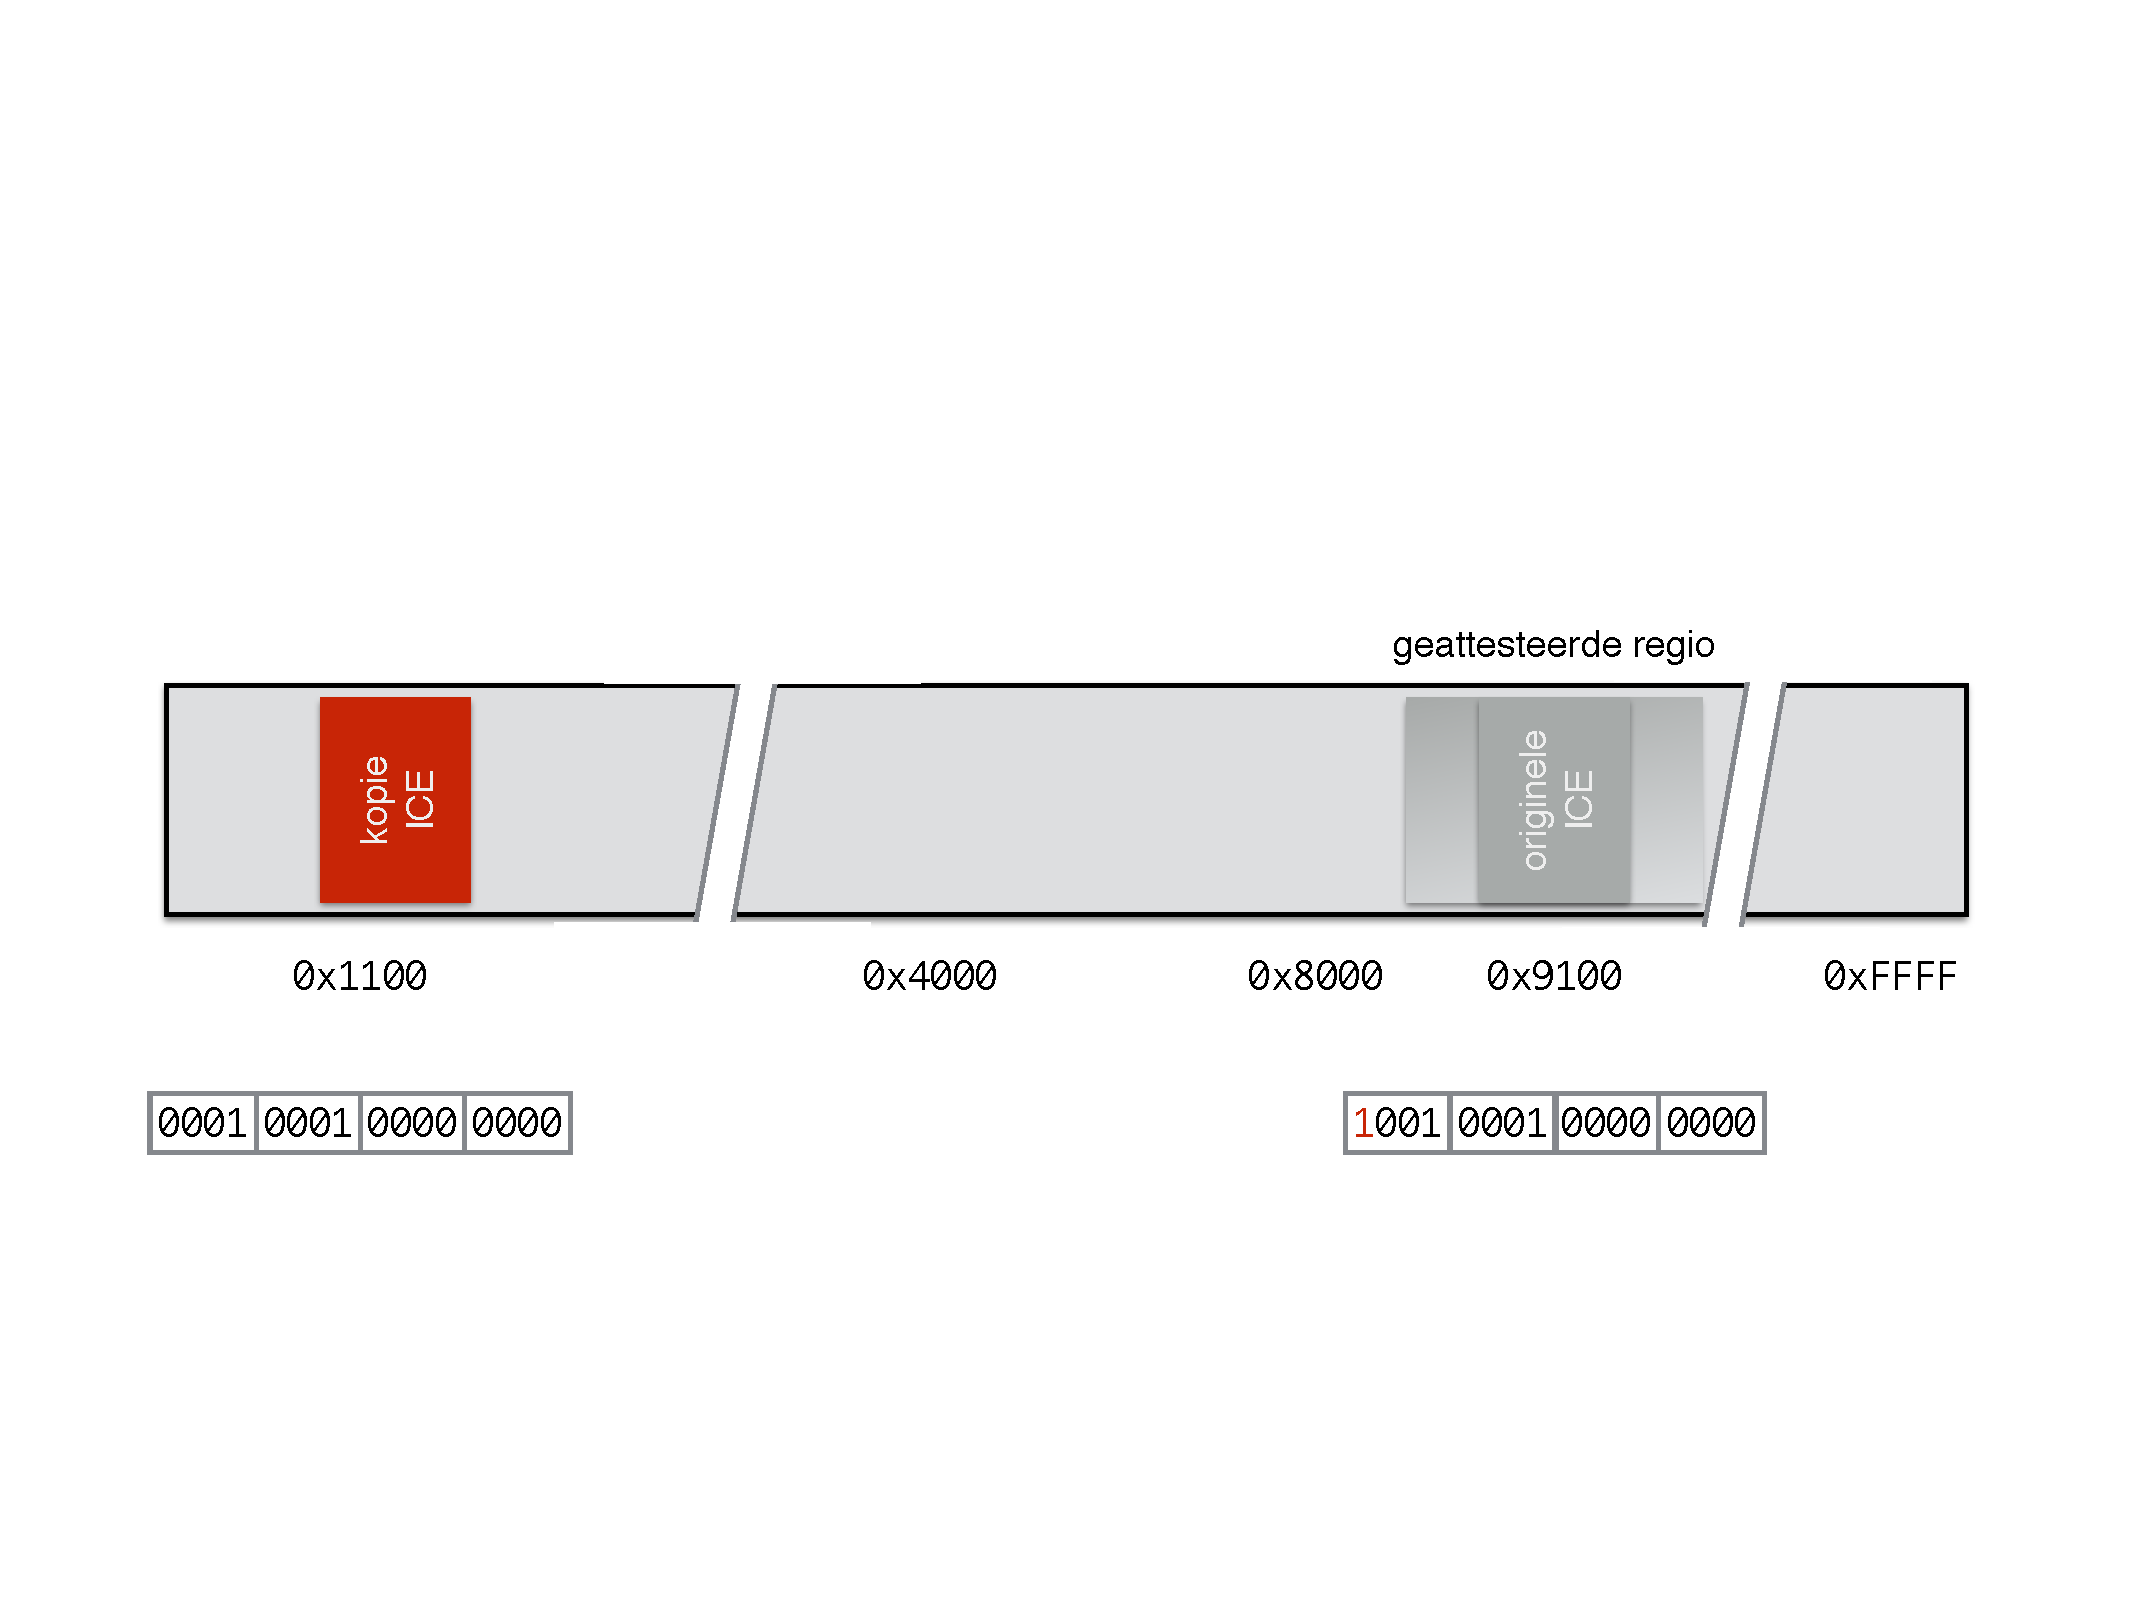
\includegraphics[width=0.9\linewidth]{resources/attestation-ice-copy.pdf}
  \caption{De legitieme ICE routine is opgeslagen op adres 0x9100 en een
  aangepaste kopie is opgeslagen op adres 0x1100. Deze twee adressen
  verschillen slechts in hun meest betekenisvolle bit. De aanvaller kan zijn
  aangepaste code gebruiken, maar nog steeds slagen voor de attestatie.}
  \label{fig:attestation-ice-copy}
\end{figure}

In \citep{perrig2010refutation} bevestigen de auteurs van ICE dat er fouten zijn
geslopen in de finale definitie van ICE en dat ze opportuniteiten hebben laten
liggen om deze aanval tegen te gaan.

\subsubsection*{Trusted Platform Module - TPM}

In bovenstaande paragrafen, lag de nadruk op het software aspect van
attestatie. Voor \mcu's, met beperkte mogelijkheden, is het belangrijk om zo
effici\"nt mogelijk om te springen met energie. Maar ook de kostprijs is een
belangrijke factor, aangezien bijkomende kosten per knoop snel kunnen oplopen
in het kader van een volledig netwerk.

Software biedt in dit laatste geval dan logischerwijs een positief economisch
antwoord. Maar het is echter ook mogelijk om voor attestatie beroep te doen op
hardware. Daar waar een eenvoudige \mcu zich nagenoeg niet kan beschermen tegen
fysieke aanvallen, is het wel mogelijk om specifieke hardware te cre\"eren die
hermetisch afgesloten is.

Een voorbeeld hiervan is de \emph{Trusted Platform Module} of TPM, van de
\emph{Trusted Platform Group}. Dit is een specificatie op industrie-niveau die
toelaat om een vertrouwen te cre\"eren tussen verschillende ge\"informatiseerde
platformen in het algemeen. Deze specificatie is in 2009 ook opgenomen als een
ISO standaard\footnote{ISO/IEC 11889-1:2009 -
\url{http://www.iso.org/iso/catalogue_detail.htm?csnumber=50970}}.

In essentie is een TPM een smart-card die in staat is om cryptografische
gegevens op te slaan en bijhorende bewerking uit te voeren, zonder dat enige
interactie van de buitenwereld kan bewerkstelligd worden en het onmogelijk is
om de opgeslagen sleutels naar buiten te exporteren. Op deze manier kan de TPM
als een initi\"eel startpunt gebruikt worden om een keten van vertrouwen op te
bouwen.

Maar een extra TPM op een reeds beladen \mcu, is soms gewoon niet mogelijk.
Daarom stelt \citep{krauss2007detecting} voor om de mogelijkheden van een TPM op
de cluster hoofden (\ref{subsection:zigbee}), afgekort tot CH, binnen het
netwerk te gebruiken. Aangezien deze per definitie voorzien zijn om meer
energie te verbruiken, kan de bijkomende kost op dit niveau verantwoord worden.

Vanuit het oogpunt dat de werking van het netwerk moet gegarandeerd worden, kan
dit tevens een interessant gegeven zijn. Knopen, of cluster nodes (CN), die de
eigenlijke metingen doen en vervolgens doorsturen via een CH, kunnen nu deze
een verzoek tot attestatie sturen.

Deze functionaliteit wordt in een eerste protocol ge\"implementeerd als het
\emph{Periodic Broadcast Attestation Protocol}, of PBAP. De aanleiding van dit
protocol is terug te vinden in de manier waarop CNs communiceren met hun CH.
Indien elke CN individueel zijn CH zou gaan attesteren, zou dit een grote
overhead leggen op de CH. Door te opteren voor het periodiek uitsturen van
attestaties, kan de CH al zijn CNs in \'e\'en keer op de hoogte stellen. Het
feit dat CNs tussen twee metingen in slaap kunnen zijn, is inherent ondervangen
door het feit dat de CHs berichten voor hun CNs bufferen.

Deze attestatie focust zich op het garanderen dat de configuratie van het CH
ongewijzigd is sinds de installatie van het netwerk. Tijdens deze installatie
zal zo'n CH met zijn TPM een keten van hashes maken en deze blokkeren in de
TPM. Dit is een techniek die \emph{sealing}\footnote{Dit is slechts \'e\'en van
de basiscomponenten van een TPM. De volledige TPM functionaliteit wordt o.a. in
\citep{parno2010bootstrapping} toegelicht in het kader van de mogelijkheden die
een TPM biedt om als initi\"ele bron van vertrouwen gebruikt te worden.}
genoemd wordt. De TPM zal deze hashes alleen vrijgeven indien deze de
configuratie van de CH kan valideren als ongewijzigd.

Door de laatste hash uit de keten van elke CH te verdelen over de CNs, wordt
het voor hen opnieuw mogelijk om boodschappen van de CH te valideren. We nemen
aan dat het CH en de CNs lichtelijk gesynchroniseerd zijn qua tijd en dat zij
de evolutie van de tijd onderling herkennen als intervallen die aangeduid wordt
met $I_\lambda$.

Indien $CH_i$ op ogenblik $I_\lambda$ inderdaad nog steeds dezelfde
configuratie heeft als initieel, zal de TPM de volgende hash uit de keten
vrijgeven: $c_{n-\lambda}^{CH_i}$\footnote{De keten was gebaseerd op de
init\"ele hash $c_0^{CH_i}$ en werd opgebouwd tot $c_n^{CH_i}$, welke
vrijgegeven werd aan de verschillende CNs.}.

De CH kan deze nieuw vrijgegeven hash nu distribueren naar de CNs, welke deze
kunnen valideren aan de hand van de vorig gekende hash:
$H(c_{n-\lambda}^{CH_i}) \overset{?}{=} c_{n-\lambda+1}^{CH_i}$. Aangezien de
CH slechts over deze hash kan beschikking indien deze is vrijgegeven door de
TPM en aangezien dit slechts gebeurd wanneer de systeem configuratie van de CH
niet gewijzigd is, heeft de CN een garantie dat de CH ongewijzigd en
betrouwbaar is.

Maar ook individuele attestaties zijn mogelijk, in de vorm van het
\emph{Individual Attestation Protocol} of IAP. Hierbij wordt er een
symmetrische encryptie sleutel $K_{CN_j,CH_i}$ gegenereerd en opgeslagen in de
TPM. De CH zal deze sleutel alleen kunnen gebruiken vanuit zijn TPM en deze zal
er slechts toegang toe verschaffen indien de configuratie van de CH ongewijzigd
is.

Een CN die nu zijn CH wil attesteren, kan nu een eenmalig en uniek getal, of
\emph{nonce}, samen mijn zijn unieke identificatie ($ID_{CN_j}$) versleutelen
en naar zijn CH sturen. Indien deze over een ongewijzigde configuratie
beschikt, zal de TPM hem toelaten om de versleutelde boodschap te decoderen en
de oorsprong van de boodschap te valideren aan de hand van $ID_{CN_j}$. De CH
kan vervolgens de \emph{nonce} opnieuw versleutelen en terug sturen naar de CN.
Deze kan tot slotte opnieuw deze boodschap decoderen en vaststellen of de CH
inderdaad dezelfde \emph{nonce} terug stuurde. Omdat de CN weet dat de CH
slechts over $K_{CN_j,CH_i}$ kan beschikken indien zijn configuratie
ongewijzigd is, beschikt de CN over voldoende aanwijzing dat de CH betrouwbaar
is.

\subsubsection*{Gedistribueerde attestatie}

In \ref{subsection:cooperation} zagen we reeds een implementatie van het Guy
Fawkes protocol, waardoor een groep van knopen toch een stemming konden houden
in het bijzijn van veroverde knopen. Een andere voorbeeld van een co\"operatief
algoritme binnen de context van software attestatie wordt voorgesteld in
\citep{yang2007distributed}. Om te vermijden dat aanvallers het lege programma
geheugen gebruiken om een kopie van de originele software van een knoop op te
slaan, wordt voordat een knoop in gebruik wordt genomen, deze lege ruimte
opgevuld met pseudo-willekeurige getallen. Dit gebeurt voor knoop $u$ op basis
van een initi\"ele waarde $S_u$, de zgn. \emph{seed}

Als knoop $u$ $n$ buren heeft, kiest $u$ $k - 1$ ($1 \leq k \leq n$)
willekeurige constante termen $a_1, a_2, \dots a_{k-1}$ uit een eindig
priemveld $Z_p$. Hiermee wordt de functie $f(x) = S_u + a_1 x+a_2 x^2 + \dots +
a_{k-1} x^{k-1}$, waarvoor evident $f(0) = S_u$. Vervolgens berekent en
verdeeld de knoop koppels van de vorm $(i,f(i))$ onder zijn buren en verwijdert
uiteindelijk $S_u$ uit zijn geheugen.

Op dit ogenblik beschikt geen enkele individuele knoop over de sleutel om de
pseudo-willekeurige inhoud van knoop $u$ opnieuw te berekenen, zelfs knoop $u$
zelf niet. Deze heeft alleen het resultaat in het geheugen staan.

De attestatie van knoop $u$ gebeurt dan als volgt: alle buren selecteren
\'e\'en knoop uit hun groep en sturen elk hun waarde $f(i)$ naar deze knoop. Op
basis van deze waarden kan via Lagrange interpolatie de functie terug opgesteld
worden en kan $S_u = f(0)$ berekend worden door deze knoop. Vervolgens kan deze
knoop knoop $u$ attesteren door het sturen van een challenge en kan deze
valideren door zelf ook deze berekening te maken.

De techniek is zonder meer interessant, maar is onderhevig aan verschillende
problemen. Zo kan een aanvaller trachten een geselecteerde knoop onder controle
te krijgen, waardoor hij in staat is om diens opnieuw samengestelde initi\"ele
waarde te bemachtigen. Nadien is hij in staat om die zelfde knoop te veroveren
en te voorzien van code die gebruik maakt van de veroverde initi\"ele waarde om
de pseudo-willekeurige getallen te generen en de lege ruimte opnieuw te
gebruiken voor zijn eigen doeleinden. De auteurs beseffen dit probleem ook en
stellen daarom een aangepast algoritme voor, dat tevens de herberekening van de
\emph{checksums} door de attesterende buren vermijdt.

In plaats van de koppels $(i, f(i))$ te versturen naar alle buren, verstuurt de
knoop nu koppels die bestaan uit een challenge en een berekende \emph{checksum}
voor die challenge: $(C_i,R_i)$. Deze worden verdeeld onder de buren, die nu
elk \'e\'en valide combinatie hebben. Wanneer een knoop nu geattesteerd wordt,
zal elk van de buren om de beurt een challenge aanbieden aan de knoop. Hierna
volgt een stem-ronde op basis van de antwoorden. De complexiteit van deze
strategie is veel hoger voor een aanvaller. Geen enkele knoop beschikt nu nog
over de initi\"ele waarde $S_u$, zelfs niet tijdelijk om de validatie te doen.
De gedistribueerde validatie berust op evenveel unieke controles als er buren
zijn. Dit zou de aanvaller verplichten om de challenge/response koppels bij elk
van de buren te veroveren om zo \'e\'en knoop te kunnen voorzien van code die
een attestatie zou kunnen weerstaan.

\subsubsection*{Conclusies en gevolgen}

Uit voorgaande paragrafen kunnen we vaststellen dat het op een eenvoudige \mcu
zeer moeilijk maar mogelijk moet zijn om een sluitende oplossing voor software
attestatie uit te realiseren. Er zijn echter veel mogelijkheden waarbij de code
van een aanvaller zich steeds tussen de verschillende stappen in de attestatie
procedure kan wringen. Zelfs indien de vaststeller rekening houdt met de tijd
die de knoop nodig heeft om de attestatie te voltooien, zijn er technieken die
snel genoeg zijn om ook hier binnen de aannemelijke grenzen te vallen. Maar al
deze ingrepen zijn zeer complex en vragen een perfecte voorbereiding.

Aan de andere kant kan voor bijna elk van deze aanvallen wel een aanpassing
toegevoegd worden aan een bestaande attestatie, zodat de aanval verijdeld kan
worden. Zoals met veel jonge beveiligings-gerelateerde wetenschappen is ook
hier het kat en muis nog lang niet gedaan en is er nog ruimte voor verder
onderzoek.

We kunnen concluderen dat software attestatie op een eenvoudige \mcu mogelijk
is, maar met de nodige omzichtigheid moet ge\"implementeerd worden.
